\documentclass[a4paper,12pt]{article}
\usepackage[a4paper, top=2cm, bottom=2cm]{geometry}
\usepackage[utf8]{vietnam}
\usepackage{textcomp, graphicx, titling, tkz-tab}
\usepackage{changepage, xcolor, amsmath, fancyvrb, minted, caption} 
\definecolor{LightGray}{gray}{0.95}

\title{\textbf{BÀI TẬP QUÁ TRÌNH 1}}
\author{\textbf{Sinh viên: Hà Huy Hoàng - MSSV: 22520460}}

\begin{document}

\maketitle
\vspace{5cm}
\section*{1. Mô tả Sokoban đã được mô hình hóa ra sao?}

\hspace*{7mm}\textbf{Trò chơi Sokoban} được xây dựng dựa trên hình tượng một nhân vật tên \textbf{Sokoban} với nhiệm vụ là đẩy các hộp vào các vị trí đích, tất nhiên là bao gồm việc không để các hộp hay nhân vật bị kẹt vào góc không thể di chuyển được. Trò chơi gồm 16 màn (\textbf{levels}) được biểu diễn bởi ma trận các kí tự, với \textbf{‘\#’} tượng trưng cho bức tường, \textbf{‘.’} là đích của các hộp cần đến, \textbf{’X’} là vị trí hộp đã tới đích, \textbf{‘ ‘} là không gian trống, \textbf{‘B’} và \textbf{‘\&’} lần lượt là vị trí các hộp và nhân vật. Tương ứng với ma trận trên thì hàm \textbf{transferToGameState2()} trong \textbf{solver.py} đã chuyển kí tự tương ứng với số (\textbf{0} là không gian trống, \textbf{1} là bức tường, \textbf{2} là vị trí nhân vật, \textbf{3} là vị trí hộp, \textbf{4} là vị trí đích các hộp cần đến, \textbf{5} là vị trí các hộp đã tới đích).\\

\textbf{Trò chơi Sokoban} có 8 cách di chuyển: 4 cách di chuyển không tương tác với hộp (\textbf{‘r’} là di chuyển nhân vật sang phải 1 ô , \textbf{‘l’} là di chuyển nhân vật sang trái 1 ô, \textbf{‘u’} là di chuyển nhân vật lên 1 ô, \textbf{‘d’} là di chuyển nhân vật xuống 1 ô) và 4 cách di chuyển tương tác với hộp (\textbf{‘R’} là di chuyển hộp và nhân vật sang phải 1 ô, \textbf{‘L’} là di chuyển hộp và nhân vật sang trái 1 ô, \textbf{‘U’} di chuyển hộp và nhân vật lên 1 ô, \textbf{‘D’} là di chuyển hộp và nhân vật xuống 1 ô)
\newpage
\subsection*{1.1.1. Trạng thái khởi đầu}
\hspace*{7mm}\textbf{Trạng thái khởi đầu} là trạng thái các hộp và nhân vật lúc bắt đầu màn chơi được lấy từ địa chỉ \textbf{.../assets/sokobanLevels/}. Trong thuật toán thì nó sẽ biểu diễn dưới dạng 1 tuple. Phần tử đầu tiên của tuple sẽ lưu vị trí bắt đầu của nhân vật, phần tử thứ hai thì sẽ lưu vị trí ban đầu của các hộp.
Lấy ví dụ về màn 1 thì trạng thái khởi đầu của nó là: \textbf{((4, 1), ((3, 2), (3, 3)))}
\begin{figure}[h]
    \begin{minipage}{0.45\textwidth}
        \centering
        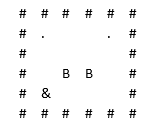
\includegraphics[width=5cm]{Level_1_text.png} 
        \caption*{\textbf{Hình 1.1.1.} Màn 1 dưới dạng text}
        \label{fig:image1}
    \end{minipage}\hfill
    \begin{minipage}{0.45\textwidth}
        \centering
        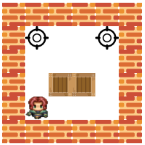
\includegraphics[width=5cm]{Level_1_render.png} 
        \caption*{\textbf{Hình 1.1.2.} Màn 1 dưới dạng ảnh}
        \label{fig:image2}
    \end{minipage}
    \centering
    \begin{minipage}{0.45\textwidth}
        \centering
        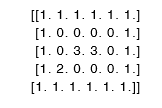
\includegraphics[width=5cm]{Level_1_num.png}
        \caption*{\textbf{Hình 1.1.3.} Màn 1 dưới dạng số}
        \label{fig:image3}
    \end{minipage}
\end{figure}
\subsection*{1.2. Trạng thái kết thúc}
\hspace*{7mm}\textbf{Trạng thái kết thúc} (hay trạng thái chiến thắng) là trạng thái tất cả các hộp đều tới đích. Trong thuật toán thì nó sẽ biểu diễn dưới dạng 1 tuple. Hai phần tử sẽ lưu vị trí cuối cùng khi kết thúc màn của nhân vật và các hộp. Việc kiểm tra xem khi nào trạng thái kết thúc sẽ thông qua hàm \textbf{isEndState()} để kiểm tra các vị trí hộp hiện tại nếu vị trí tất cả các hộp (posBox) và tất cả các đích (posGoals) đều giống nhau thì khi ấy sẽ là trạng thái kết thúc. Lấy vị dụ màn 1 với thuật toán BFS thì trạng thái kết thúc sẽ có giá trị là: \textbf{((1, 2), ((1, 4), (1, 1)))}
\begin{figure}[h]
\centering
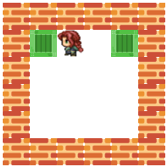
\includegraphics[width=4cm]{Level_1_end.png}
\caption*{\textbf{Hình 1.2.} Màn 1 khi kết thúc (chiến thắng) dùng BFS}
\end{figure}
\newpage
\subsection*{1.3. Không gian trạng thái}
\hspace*{7mm}\textbf{Không gian trạng thái} là không gian lưu trữ tất cả trạng thái của nhân vật và các hộp (kể cả trạng thái bắt đầu lẫn trạng thái kết thúc). Trong thuật toán thì nó cũng lưu dưới dạng tuple chứa nhiều trạng thái khác nhau. Trong màn 1 khi dùng BFS thì không gian trạng thái sẽ là \textbf{[((4, 1), ((3, 2), (3, 3))), ((4, 2), ((3, 2), (3, 3))), ((3, 2), ((3, 3), (2, 2))), ((2, 2), ((3, 3), (1, 2))), ((3, 2), ((3, 3), (1, 2))), ((3, 3), ((1, 2), (3, 4))), ((4, 3), ((1, 2), (3, 4))), ((4, 4), ((1, 2), (3, 4))), ((3, 4), ((1, 2), (2, 4))), ((2, 4), ((1, 2), (1, 4))), ((2, 3), ((1, 2), (1, 4))), ((1, 3), ((1, 2), (1, 4))), ((1, 2), ((1, 4), (1, 1)))]}
\begin{figure}[h]
    \centering
    \begin{minipage}{0.2\textwidth}
        \centering
        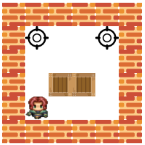
\includegraphics[width=3cm]{Level_1_render.png} 
        \label{fig:image1}
    \end{minipage}
    \begin{minipage}{0.2\textwidth}
        \centering
        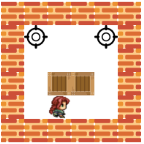
\includegraphics[width=3cm]{Level_1.1.png} 
        \label{fig:image2}
    \end{minipage}
    \begin{minipage}{0.2\textwidth}
        \centering
        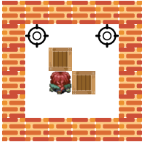
\includegraphics[width=3cm]{Level_1.2.png} 
        \label{fig:image3}
    \end{minipage}
    $\cdots$
    \begin{minipage}{0.2\textwidth}
        \centering
        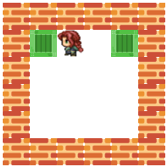
\includegraphics[width=3cm]{Level_1_end.png}
        \label{fig:image4}
    \end{minipage}
    \caption*{\textbf{Hình 1.3.} Không gian trạng thái của màn 1 khi dùng BFS}
\end{figure}
\subsection*{1.4. Các hành động hợp lệ}
\hspace*{7mm}\textbf{Các hành động hợp lệ} là các hành động có thể thực hiện trong một trạng thái nào đó bao gồm di chuyển tương tác với hộp và di chuyển không tương tác với hộp. Ví dụ khi màn 1 bắt đầu thì nhân vật chỉ có hai hướng di chuyển: 1 là đi sang phải 1 ô, 2 là đi lên trên 1 ô. Các hành động này được lưu trong một tuple dựa trên vị trí của nhân vật và các hộp tại trạng thái hiện tại thông qua hàm \textbf{legalActions()}. Lúc màn 1 bắt đầu thì sẽ trả về: \textbf{((-1, 0, 'u'), (0, 1, 'r'))}
\begin{figure}[h]
\centering
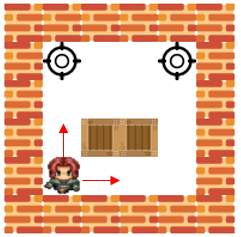
\includegraphics[width=4cm]{Level_1_actions.png}
\caption*{\textbf{Hình 1.4.} Các hành động hợp lệ khi màn 1 bắt đầu}
\end{figure}
\subsection*{1.5. Hàm tiến triển (successor function) là gì?}
Hàm tiến triển trong trường hợp này là hàm \textbf{updateState()}, có tác dụng dùng để cập nhật lại trạng thái của nhân vật hiện tượng sau khi thực hiện một hành động.
\newpage
\section*{2. DFS/BFS/UCS cho Sokoban}
% \begin{figure}[h]
% \centering
% \includegraphics[width=15cm]{Bảng 1.png}
% \caption*{\textbf{Hình 2.1.} Bảng thống kê về số đường đi của 3 thuật toán}
% \end{figure}
% \begin{figure}[h]
% \centering
% \includegraphics[width=15cm]{Bảng 2.png}
% \caption*{\textbf{Hình 2.2.} Bảng thống kê về thời gian chạy của 3 thuật toán}
% \end{figure}


\begin{table}[ht]
\begin{minipage}[b]{0.45\linewidth}
\centering
\begin{tabular}{|c|c|c|c|}
\hline
Màn & DFS & BFS & UCS \\
\hline
1 & 79 & 12 & 12 \\
2 & 24 & 9 & 9 \\
3 & 403 & 15 & 15 \\
4 & 27 & 7 & 7 \\
5 & - & 20 & 20 \\
6 & 55 & 19 & 19 \\
7 & 707 & 21 & 21 \\
8 & 323 & 97 & 97 \\
9 & 74 & 8 & 8 \\
10 & 37 & 33 & 33 \\
11 & 36 & 34 & 34 \\
12 & 109 & 23 & 23 \\
13 & 185 & 31 & 31 \\
14 & 865 & 23 & 23 \\
15 & 291 & 105 & 105 \\
16 & - & 34 & 34 \\
\hline
\end{tabular}
\caption*{\textbf{Bảng 1.} Bảng thống kê số đường đi}
\end{minipage}
\hspace{0.5cm}
\begin{minipage}[b]{0.45\linewidth}
\centering
\begin{tabular}{|c|c|c|c|}
\hline
Màn & DFS & BFS & UCS \\
\hline
1 & 0.14s & 0.26s & 0.23s \\
2 & 0.01s & 0.03s & 0.04s \\
3 & 0.44s & 0.33s & 0.27s \\
4 & 0.01s & 0.03s & 0.03s \\
5 & - & 279.39s & 225.16s \\
6 & 0.07s & 0.06s & 0.08s \\
7 & 1.23s & 1.42s & 1.18s \\
8 & 0.16s & 0.38s & 0.42s \\
9 & 0.48s & 0.05s & 0.06s \\
10 & 0.06s & 0.07s & 0.04s \\
11 & 0.09s & 0.07s & 0.08s \\
12 & 0.26s & 0.24s & 0.21s \\
13 & 0.33s & 0.27s & 0.43s \\
14 & 6.16s & 4.26s & 5.89s \\
15 & 0.32s & 0.5s & 0.6s \\
16 & - & 34.84s & 34.89s \\
\hline
\end{tabular}
\caption*{\textbf{Bảng 2.} Bảng thống kê thời gian giải}
\end{minipage}
\end{table}

\textbf{Ghi chú:} Màn 5 và màn 16 em không chạy được ạ (đã ngồi đợi hơn 1 tiếng) 

\subsection*{2.1 DFS}
 \hspace*{7mm}Ta có thể nhận thấy rằng thuật toán DFS thường hoàn thành màn chơi với số bước đi lớn hơn đáng kể so với hai thuật toán còn lại, tuy nhiên thời gian thực hiện không chênh lệch nhiều, thậm chí có thể nhỉnh hơn hai thuật toán còn lại. NHiện tượng này là do DFS tập trung chủ yếu vào việc tìm ra lời giải mà không quan tâm đến số lượng bước đi, chỉ cần khi duyệt qua các nhánh một cách sâu nhất có thể và tìm lời giải.
\subsection*{2.2 BFS}
\hspace*{7mm}Thuật toán này có lời giải đường đi ít bước ngang với UCS nhưng tốn nhiều bộ nhớ nhất để lưu trữ các trạng thái được mở rộng. Nhưng nhìn chung đây là một thuật toán hiệu quả đối với trò chơi Sokoban khi mà mỗi bước đi chỉ được đi 1 bước. 
\subsection*{2.3 UCS}
\hspace*{7mm}Thuật toán này là sự kết hợp của dfs và bfs khi mà nó mở rộng trạng thái bằng cách ưu tiên xét những đường đi (số bước đi mà không di chuyển hộp) có chi phí bé nhất. Nên lời giải của bài toán này sẽ được những bước đi mà không di chuyển hộp ngắn hơn nhiều so với DFS.\\
\\
\newpage
\hspace*{7mm} Về cơ bản trong trường hợp của bài toán Sokoban này, UCS và BFS đều sẽ là sự lựa chọn tốt hơn so với DFS. Thường trong các trường hợp của bài toán tìm đường thì UCS sẽ tối ưu hơn BFS vì chi phí mỗi bước đi sẽ khác nhau nhưng trong bài này chi phí mỗi bước đi là như nhau nên bài này hiệu suất của BFS và UCS là gần như tương đương nhau.\\
\\
\hspace*{7mm} Đối với bài toán này khi sử dụng DFS, BFS, UCS thì màn 15 là khó nhất vì số bước đi trong khi dùng BFS hoặc UCS (không tính DFS vì nó không tối ưu được số đường đi). Thời gian màn 5 có thể chạy lâu nhất (DFS còn không chạy nổi) nhưng chỉ bởi vì không gian trạng thái nó là lớn nhất trong tất cả các màn (kích thước rộng và ít tường ngăn) chứ không phải vì nó khó giải và phức tạp về đường đi.
\end{document}